\section{Process API}

\textbf{Execution Model -- Assembler (simplified)}
\begin{items}
  \item OS interacts directly with compiled programs \\*
    - switch between processes/threads \( \leadsto \) \textbf{save}/\textbf{restore} state \\*
    - deal with/pass on \textbf{signals}/\textbf{exceptions} \\*
    - receive \textbf{requests} from applications
  \item \underline{Instructions}: \\*
    - \code{mov}: Copy referenced data from second operand to first operand \\*
    - \code{add}/\code{sub}/\code{mul}/\code{div}: Add,\dots from second operand to first operand \\*
    - \code{inc}/\code{dec}: increment/decrement register/memory location \\*
    - \code{shl}/\code{shr}: shift first operand left/right by amount given by second operand \\*
    - \code{and}/\code{or}/\code{xor}: calculate bitwise and,\dots of two operands storing result in first \\*
    - \code{not}: bitwise negate operand
\end{items}

\ \\
\textbf{Execution Model -- Stack (x86)}
\begin{items}
  \item \underline{stack pointer} (SP): holds address of stack top (growing downwards)
  \item \underline{stack frames}: larger stack chunks
  \item \underline{base pointer} (BP): used to organize stack frames
\end{items}

\begin{figure}[H]\centering\label{Stack}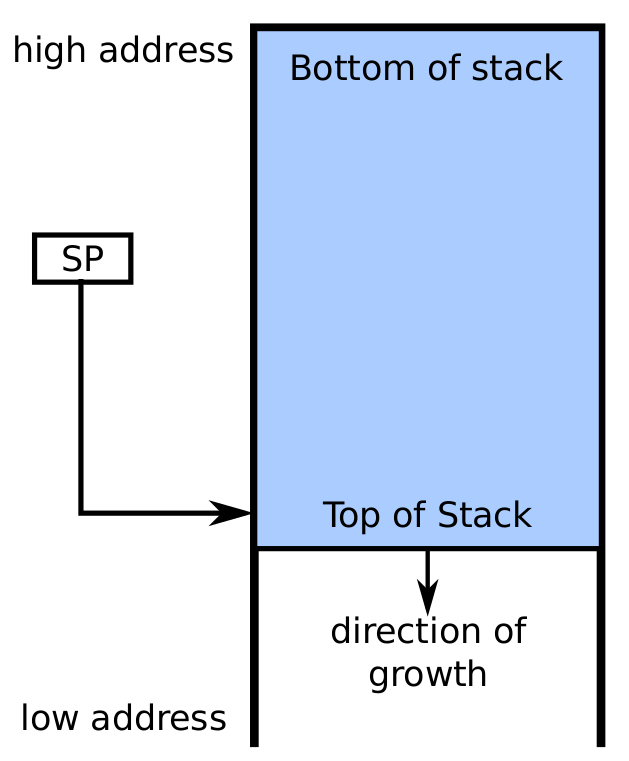
\includegraphics[width=0.2\textwidth]{Stack}\end{figure}

\ \\
\textbf{Execution Model -- jump/branch/call commands (x86)}
\begin{items}
  \item \code{jmp}: continue execution at operand address
  \item \code{j\$condition}: jump depending on PSW content \\*
    true \( \leadsto \) jump \\*
    false \( \leadsto \) continue \\*
    examples: \code{je} (jump equal), \code{jz} (jump zero)
  \item \code{call}: push function to stack and jump to it
  \item \code{return}: return from function (jump to return address)
\end{items}

\ \\
\textbf{Execution Model -- Application Binary Interface (ABI)}
\begin{items}
  \item standardizes binary interface between programs, modules, OS: \\*
    - executable/object file layout \\*
    - calling conventions \\*
    - alignment rules
  \item \underline{calling conventions}: standardize exact way function calls are implemented \\*
    \( \leadsto \) interoperability between compilers
\end{items}

\textbf{Execution Model -- calling conventions (x86)}
\begin{items}
  \item function call (caller):
  \begin{enumeration}
    \item save local scope state 
    \item set up parameters where function can find them
    \item transfer control flow
  \end{enumeration}
  \item function call (called function):
  \begin{enumeration}
    \item set up new local scope (local variables)
    \item perform duty
    \item put return value where caller can find it
    \item jump back to caller (IP)
  \end{enumeration}
\end{items}

\textbf{Passing parameters to the system}
\begin{items}
  \item parameters are passed through \textbf{system calls}
  \item call number + specific parameters must be passed
  \item parameters can be transferred through \\*
    - \underline{CPU registers} (\textasciitilde 6) \\*
    - \underline{Main Memory} (heap/stack -- more parameters, data types)
  \item ABI specifies how to pass parameters
  \item \underline{return code} needs to be returned to application \\*
    - \textbf{negative}: error code \\*
    - \textbf{positive + 0}: success \\*
    - usually returned via A+D registers
\end{items}

\textbf{System call handler}
\begin{items}
  \item implements the actual serivce called through a syscall:
  \begin{enumeration}
    \item saves tainted registers
    \item reads passed parameters
    \item sanitizes/checks parameters
    \item checks if caller has enough permissions to perform the requested action
    \item performs requested action in behalf of the caller
    \item returns to caller with success/error code
  \end{enumeration}
\end{items}

\textbf{Process API -- creation}
\begin{items}
  \item process creation events:
  \begin{enumeration}
    \item system initialization
    \item process creation syscall
    \item user requests process creation
    \item batch job-initiation
  \end{enumeration}
  \item events map to two mechanisms:
  \begin{enumeration}
    \item Kernel spawns initial user space process on boot (Linux: \code{init})
    \item User space processes can spawn other processes (within their quota)
  \end{enumeration}
\end{items}

\textbf{Process API -- creation (POSIX)}
\begin{items}
  \item \code{PID}: identifies process
  \item \code{pid = fork()}: duplicates current process: \\*
    returns \code{0} to new child \\*
    returns new \code{PID} to parent \\*
    \( \leadsto \) child and parent independent after \code{fork}
  \item \code{exec(name)}: replaces own memory based on executable file \\*
    \code{name} specifies binary executable file
  \item \code{exit(status)}: terminates process, returns \code{status}
  \item \code{pid = waitpid(pid, \&status)}: wait for child termination \\*
    - \code{pid}: process to wait for \\*
    - \code{status}: points to data structure that returns information about the process \\* \phantom{- \code{status}:} (e.g., exit status) \\*
    - passed \code{pid} is returned on success, \code{-1} otherwise
  \item \underline{process tree}: processes create child processes, which create child processes, \dots \\*
    - parent and child execute concurrently \\*
    - parent waits for child to terminate (collecting the exit state)
\end{items}

\textbf{Daemons}
\begin{items}
  \item = program designed to run in the background
  \item detached from parent process after creation, reattached to process tree root (\code{init})
\end{items}

\textbf{Process States}
\begin{items}
  \item \underline{blocking}: process does nothing but wait \\*
    - usually happens on syscalls (OS doesn't run process until event happens)
\end{items}

\begin{figure}[H]\centering\label{ProcessState}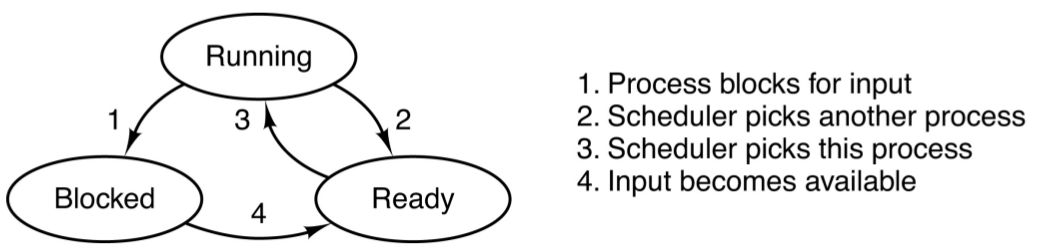
\includegraphics[width=0.4\textwidth]{ProcessState}\end{figure}

\textbf{Process Termination}
\begin{items}
  \item different termination events: 
  \begin{enumeration}
    \item normal exit (voluntary) \\*
      - \code{return 0} at end of \code{main} \\*
      - \code{exit(0)}
    \item error exit (voluntary) \\*
      - \code{return x} (\code{x} \( \neq 0 \)) at end of \code{main} \\*
      - \code{exit(x)} (\code{x} \( \neq 0 \)) \\*
      - \code{abort()}
    \item fatal error (involuntary) \\*
      - OS kills process after exception \\*
      - process exceeds allowed ressources
    \item killed by another process (involuntary) \\*
      - another process sends kill signal (only as parent process or administrator)
  \end{enumeration}
\end{items}

\textbf{Exit Status}
\begin{items}
  \item voluntary exit: process returns exit status (integer)
  \item ressources not completely free'd after process terminates \\*
    \( \leadsto \) \textbf{Zombie} or \textbf{process stub} (contains exit status until collected via \code{waitpid})
  \item \underline{Orphans}: Processes without parents \\*
    - usually adopted by \code{init} \\*
    - some systems kill all children when parent is killed
  \item exit status on involuntary exit: \\*
    - Bits \code{0-6}: signal number that killed process (\code{0} on normal exit) \\*
    - Bit \code{7}: set if process was killed by signal \\*
    - Bits \code{8-15}: \code{0} if killed by signal (exit status on normal exit)
\end{items}
